
%% bare_conf.tex
%% V1.4b
%% 2015/08/26
%% by Michael Shell
%% See:
%% http://www.michaelshell.org/
%% for current contact information.
%%
%% This is a skeleton file demonstrating the use of IEEEtran.cls
%% (requires IEEEtran.cls version 1.8b or later) with an IEEE
%% conference paper.
%%
%% Support sites:
%% http://www.michaelshell.org/tex/ieeetran/
%% http://www.ctan.org/pkg/ieeetran
%% and
%% http://www.ieee.org/

%%*************************************************************************
%% Legal Notice:
%% This code is offered as-is without any warranty either expressed or
%% implied; without even the implied warranty of MERCHANTABILITY or
%% FITNESS FOR A PARTICULAR PURPOSE! 
%% User assumes all risk.
%% In no event shall the IEEE or any contributor to this code be liable for
%% any damages or losses, including, but not limited to, incidental,
%% consequential, or any other damages, resulting from the use or misuse
%% of any information contained here.
%%
%% All comments are the opinions of their respective authors and are not
%% necessarily endorsed by the IEEE.
%%
%% This work is distributed under the LaTeX Project Public License (LPPL)
%% ( http://www.latex-project.org/ ) version 1.3, and may be freely used,
%% distributed and modified. A copy of the LPPL, version 1.3, is included
%% in the base LaTeX documentation of all distributions of LaTeX released
%% 2003/12/01 or later.
%% Retain all contribution notices and credits.
%% ** Modified files should be clearly indicated as such, including  **
%% ** renaming them and changing author support contact information. **
%%*************************************************************************


% *** Authors should verify (and, if needed, correct) their LaTeX system  ***
% *** with the testflow diagnostic prior to trusting their LaTeX platform ***
% *** with production work. The IEEE's font choices and paper sizes can   ***
% *** trigger bugs that do not appear when using other class files.       ***                          ***
% The testflow support page is at:
% http://www.michaelshell.org/tex/testflow/



\documentclass[onecolumn,draftcls,a4paper,compsoc]{IEEEtran}
% Some Computer Society conferences also require the compsoc mode option,
% but others use the standard conference format.
%
% If IEEEtran.cls has not been installed into the LaTeX system files,
% manually specify the path to it like:
% \documentclass[conference]{../sty/IEEEtran}


% *** STUFF WE ADD THAT THE PACKAGE SHOULD HAVE HAD ***

\usepackage{amsmath}
\usepackage{hyperref}
\usepackage{cleveref}



% Some very useful LaTeX packages include:
% (uncomment the ones you want to load)


% *** MISC UTILITY PACKAGES ***
%
%\usepackage{ifpdf}
% Heiko Oberdiek's ifpdf.sty is very useful if you need conditional
% compilation based on whether the output is pdf or dvi.
% usage:
% \ifpdf
%   % pdf code
% \else
%   % dvi code
% \fi
% The latest version of ifpdf.sty can be obtained from:
% http://www.ctan.org/pkg/ifpdf
% Also, note that IEEEtran.cls V1.7 and later provides a builtin
% \ifCLASSINFOpdf conditional that works the same way.
% When switching from latex to pdflatex and vice-versa, the compiler may
% have to be run twice to clear warning/error messages.






% *** CITATION PACKAGES ***
%
%\usepackage{cite}
% cite.sty was written by Donald Arseneau
% V1.6 and later of IEEEtran pre-defines the format of the cite.sty package
% \cite{} output to follow that of the IEEE. Loading the cite package will
% result in citation numbers being automatically sorted and properly
% "compressed/ranged". e.g., [1], [9], [2], [7], [5], [6] without using
% cite.sty will become [1], [2], [5]--[7], [9] using cite.sty. cite.sty's
% \cite will automatically add leading space, if needed. Use cite.sty's
% noadjust option (cite.sty V3.8 and later) if you want to turn this off
% such as if a citation ever needs to be enclosed in parenthesis.
% cite.sty is already installed on most LaTeX systems. Be sure and use
% version 5.0 (2009-03-20) and later if using hyperref.sty.
% The latest version can be obtained at:
% http://www.ctan.org/pkg/cite
% The documentation is contained in the cite.sty file itself.






% *** GRAPHICS RELATED PACKAGES ***
%
\ifCLASSINFOpdf
   \usepackage[pdftex]{graphicx}
  % declare the path(s) where your graphic files are
  % \graphicspath{{../pdf/}{../jpeg/}}
  % and their extensions so you won't have to specify these with
  % every instance of \includegraphics
  % \DeclareGraphicsExtensions{.pdf,.jpeg,.png}
\else
  % or other class option (dvipsone, dvipdf, if not using dvips). graphicx
  % will default to the driver specified in the system graphics.cfg if no
  % driver is specified.
  % \usepackage[dvips]{graphicx}
  % declare the path(s) where your graphic files are
  % \graphicspath{{../eps/}}
  % and their extensions so you won't have to specify these with
  % every instance of \includegraphics
  % \DeclareGraphicsExtensions{.eps}
\fi
% graphicx was written by David Carlisle and Sebastian Rahtz. It is
% required if you want graphics, photos, etc. graphicx.sty is already
% installed on most LaTeX systems. The latest version and documentation
% can be obtained at: 
% http://www.ctan.org/pkg/graphicx
% Another good source of documentation is "Using Imported Graphics in
% LaTeX2e" by Keith Reckdahl which can be found at:
% http://www.ctan.org/pkg/epslatex
%
% latex, and pdflatex in dvi mode, support graphics in encapsulated
% postscript (.eps) format. pdflatex in pdf mode supports graphics
% in .pdf, .jpeg, .png and .mps (metapost) formats. Users should ensure
% that all non-photo figures use a vector format (.eps, .pdf, .mps) and
% not a bitmapped formats (.jpeg, .png). The IEEE frowns on bitmapped formats
% which can result in "jaggedy"/blurry rendering of lines and letters as
% well as large increases in file sizes.
%
% You can find documentation about the pdfTeX application at:
% http://www.tug.org/applications/pdftex





% *** MATH PACKAGES ***
%
\usepackage{amsmath}
\usepackage{amsfonts}
\usepackage{amssymb}
\usepackage{blkarray}
\usepackage{kbordermatrix}
\renewcommand{\kbldelim}{[}% Left delimiter
\renewcommand{\kbrdelim}{]}% Right delimiter
% A popular package from the American Mathematical Society that provides
% many useful and powerful commands for dealing with mathematics.
%
% Note that the amsmath package sets \interdisplaylinepenalty to 10000
% thus preventing page breaks from occurring within multiline equations. Use:
%\interdisplaylinepenalty=2500
% after loading amsmath to restore such page breaks as IEEEtran.cls normally
% does. amsmath.sty is already installed on most LaTeX systems. The latest
% version and documentation can be obtained at:
% http://www.ctan.org/pkg/amsmath





% *** SPECIALIZED LIST PACKAGES ***
%
%\usepackage{algorithmic}
% algorithmic.sty was written by Peter Williams and Rogerio Brito.
% This package provides an algorithmic environment fo describing algorithms.
% You can use the algorithmic environment in-text or within a figure
% environment to provide for a floating algorithm. Do NOT use the algorithm
% floating environment provided by algorithm.sty (by the same authors) or
% algorithm2e.sty (by Christophe Fiorio) as the IEEE does not use dedicated
% algorithm float types and packages that provide these will not provide
% correct IEEE style captions. The latest version and documentation of
% algorithmic.sty can be obtained at:
% http://www.ctan.org/pkg/algorithms
% Also of interest may be the (relatively newer and more customizable)
% algorithmicx.sty package by Szasz Janos:
% http://www.ctan.org/pkg/algorithmicx




% *** ALIGNMENT PACKAGES ***
%
%\usepackage{array}
% Frank Mittelbach's and David Carlisle's array.sty patches and improves
% the standard LaTeX2e array and tabular environments to provide better
% appearance and additional user controls. As the default LaTeX2e table
% generation code is lacking to the point of almost being broken with
% respect to the quality of the end results, all users are strongly
% advised to use an enhanced (at the very least that provided by array.sty)
% set of table tools. array.sty is already installed on most systems. The
% latest version and documentation can be obtained at:
% http://www.ctan.org/pkg/array


% IEEEtran contains the IEEEeqnarray family of commands that can be used to
% generate multiline equations as well as matrices, tables, etc., of high
% quality.




% *** SUBFIGURE PACKAGES ***
%\ifCLASSOPTIONcompsoc
%  \usepackage[caption=false,font=normalsize,labelfont=sf,textfont=sf]{subfig}
%\else
%  \usepackage[caption=false,font=footnotesize]{subfig}
%\fi
% subfig.sty, written by Steven Douglas Cochran, is the modern replacement
% for subfigure.sty, the latter of which is no longer maintained and is
% incompatible with some LaTeX packages including fixltx2e. However,
% subfig.sty requires and automatically loads Axel Sommerfeldt's caption.sty
% which will override IEEEtran.cls' handling of captions and this will result
% in non-IEEE style figure/table captions. To prevent this problem, be sure
% and invoke subfig.sty's "caption=false" package option (available since
% subfig.sty version 1.3, 2005/06/28) as this is will preserve IEEEtran.cls
% handling of captions.
% Note that the Computer Society format requires a larger sans serif font
% than the serif footnote size font used in traditional IEEE formatting
% and thus the need to invoke different subfig.sty package options depending
% on whether compsoc mode has been enabled.
%
% The latest version and documentation of subfig.sty can be obtained at:
% http://www.ctan.org/pkg/subfig




% *** FLOAT PACKAGES ***
%
%\usepackage{fixltx2e}
% fixltx2e, the successor to the earlier fix2col.sty, was written by
% Frank Mittelbach and David Carlisle. This package corrects a few problems
% in the LaTeX2e kernel, the most notable of which is that in current
% LaTeX2e releases, the ordering of single and double column floats is not
% guaranteed to be preserved. Thus, an unpatched LaTeX2e can allow a
% single column figure to be placed prior to an earlier double column
% figure.
% Be aware that LaTeX2e kernels dated 2015 and later have fixltx2e.sty's
% corrections already built into the system in which case a warning will
% be issued if an attempt is made to load fixltx2e.sty as it is no longer
% needed.
% The latest version and documentation can be found at:
% http://www.ctan.org/pkg/fixltx2e


%\usepackage{stfloats}
% stfloats.sty was written by Sigitas Tolusis. This package gives LaTeX2e
% the ability to do double column floats at the bottom of the page as well
% as the top. (e.g., "\begin{figure*}[!b]" is not normally possible in
% LaTeX2e). It also provides a command:
%\fnbelowfloat
% to enable the placement of footnotes below bottom floats (the standard
% LaTeX2e kernel puts them above bottom floats). This is an invasive package
% which rewrites many portions of the LaTeX2e float routines. It may not work
% with other packages that modify the LaTeX2e float routines. The latest
% version and documentation can be obtained at:
% http://www.ctan.org/pkg/stfloats
% Do not use the stfloats baselinefloat ability as the IEEE does not allow
% \baselineskip to stretch. Authors submitting work to the IEEE should note
% that the IEEE rarely uses double column equations and that authors should try
% to avoid such use. Do not be tempted to use the cuted.sty or midfloat.sty
% packages (also by Sigitas Tolusis) as the IEEE does not format its papers in
% such ways.
% Do not attempt to use stfloats with fixltx2e as they are incompatible.
% Instead, use Morten Hogholm'a dblfloatfix which combines the features
% of both fixltx2e and stfloats:
%
% \usepackage{dblfloatfix}
% The latest version can be found at:
% http://www.ctan.org/pkg/dblfloatfix




% *** PDF, URL AND HYPERLINK PACKAGES ***
%
%\usepackage{url}
% url.sty was written by Donald Arseneau. It provides better support for
% handling and breaking URLs. url.sty is already installed on most LaTeX
% systems. The latest version and documentation can be obtained at:
% http://www.ctan.org/pkg/url
% Basically, \url{my_url_here}.




% *** Do not adjust lengths that control margins, column widths, etc. ***
% *** Do not use packages that alter fonts (such as pslatex).         ***
% There should be no need to do such things with IEEEtran.cls V1.6 and later.
% (Unless specifically asked to do so by the journal or conference you plan
% to submit to, of course. )

% Allow larger bmatrix width
\setcounter{MaxMatrixCols}{20} %Set max column to 20

% correct bad hyphenation here
\hyphenation{op-tical net-works semi-conduc-tor}

% Include SI units
\usepackage{siunitx}

\begin{document}
%
% paper title
% Titles are generally capitalized except for words such as a, an, and, as,
% at, but, by, for, in, nor, of, on, or, the, to and up, which are usually
% not capitalized unless they are the first or last word of the title.
% Linebreaks \\ can be used within to get better formatting as desired.
% Do not put math or special symbols in the title.
\title{Bare Demo of IEEEtran.cls\\ for IEEE Conferences}


% author names and affiliations
% use a multiple column layout for up to three different
% affiliations
\author{\IEEEauthorblockN{CA7 Group 733} \\
\IEEEauthorblockA{Technical Faculty of IT and Design \\
Department of Control and Automation \\
Frederik Bajers Vej 7C \\
9220 Aalborg East \\
Email: \href{mailto:es-21-ca-7-733@student.aau.dk}{es-21-ca-7-733@student.aau.dk}}
}

% conference papers do not typically use \thanks and this command
% is locked out in conference mode. If really needed, such as for
% the acknowledgment of grants, issue a \IEEEoverridecommandlockouts
% after \documentclass

% for over three affiliations, or if they all won't fit within the width
% of the page, use this alternative format:
% 
%\author{\IEEEauthorblockN{Michael Shell\IEEEauthorrefmark{1},
%Homer Simpson\IEEEauthorrefmark{2},
%James Kirk\IEEEauthorrefmark{3}, 
%Montgomery Scott\IEEEauthorrefmark{3} and
%Eldon Tyrell\IEEEauthorrefmark{4}}
%\IEEEauthorblockA{\IEEEauthorrefmark{1}School of Electrical and Computer Engineering\\
%Georgia Institute of Technology,
%Atlanta, Georgia 30332--0250\\ Email: see http://www.michaelshell.org/contact.html}
%\IEEEauthorblockA{\IEEEauthorrefmark{2}Twentieth Century Fox, Springfield, USA\\
%Email: homer@thesimpsons.com}
%\IEEEauthorblockA{\IEEEauthorrefmark{3}Starfleet Academy, San Francisco, California 96678-2391\\
%Telephone: (800) 555--1212, Fax: (888) 555--1212}
%\IEEEauthorblockA{\IEEEauthorrefmark{4}Tyrell Inc., 123 Replicant Street, Los Angeles, California 90210--4321}}




% use for special paper notices
%\IEEEspecialpapernotice{(Invited Paper)}

% Setup for use of lemmas and theorems

\newtheorem{theorem}{Theorem}[section]
\newtheorem{corollary}{Corollary}[theorem]
\newtheorem{lemma}[theorem]{Lemma}


% make the title area
\maketitle

% As a general rule, do not put math, special symbols or citations
% in the abstract
\begin{abstract}
The abstract goes here.
\end{abstract}

% no keywords




% For peer review papers, you can put extra information on the cover
% page as needed:
% \ifCLASSOPTIONpeerreview
% \begin{center} \bfseries EDICS Category: 3-BBND \end{center}
% \fi
%
% For peerreview papers, this IEEEtran command inserts a page break and
% creates the second title. It will be ignored for other modes.
\IEEEpeerreviewmaketitle



\section{Introduction}

Put introduction here



\section{Graph Theory}\label{sec:GraphTheory}

\subsection{System modelling }
This section describes the interconnected component in a water distributed network (WDN) using Graph Theory. Furthermore thee component classes will be examined, ie. pipes, pumps and valves.


\subsection{Graph Theory}
When using graph theory as an analytical tool the incident matrix $H$ comes in handy when describing the connection between edges and nodes. The $H$ matrix is defined as follows: 

\subsubsection{The Incident Matrix}
\begin{equation}
	H_{i,j} = \begin{cases}
		-1 & \text{If the $j^{th}$ edge enters the $i^{th}$ node} \\
		0 & \text{If the $j^{th}$ edge is not connected to the $i^{th}$ node} \\
		1 & \text{If the $j^{th}$ edge s leaving the $i^{th}$ node}
	\end{cases}
\end{equation} %Description of the incident matrix

\subsubsection{Spanning Tree}
The spanning tree is the connected graph but with no loops, i.e you can not find a route around the graph where you start and end in the same node without entering a node more than one time. 
When adding one chord to the graph, exactly one loop is created.


\subsubsection{The Loop Marix}
The definition of a loop is a unique route along the edges of the graph network, where all nodes are unique except the end node - In a loop the end node must also be the start node.

The loop-matrix can be calculated in one of two ways. The first one is shown in the equation below

\begin{equation}\label{eq:LoopMatrix}
	B = \begin{bmatrix}
		I & -\bar{H}_{C}^{T}\cdot\bar{H}_{T}^{-T}
	\end{bmatrix}
\end{equation}


With $\bar{H}_{C}$ being the matrix containing only chord columns of the incident matrix. The same goes for  $\bar{H}_{T}$, containing only the non-chord columns. The bar indicates that the row corresponding to the reference node has been removed from the incident matrix.

The other method is more graphical but can be formulated as follows: 

Adding one chord to the spanning tree, creates exactly one loop. Writing up the edges in the loop, with signs corresponing to the incident matrix creates a row in the loop matrix $ B $. 


\newpage
\subsection{Simplified system}
\begin{figure}[h!]
	\centering
	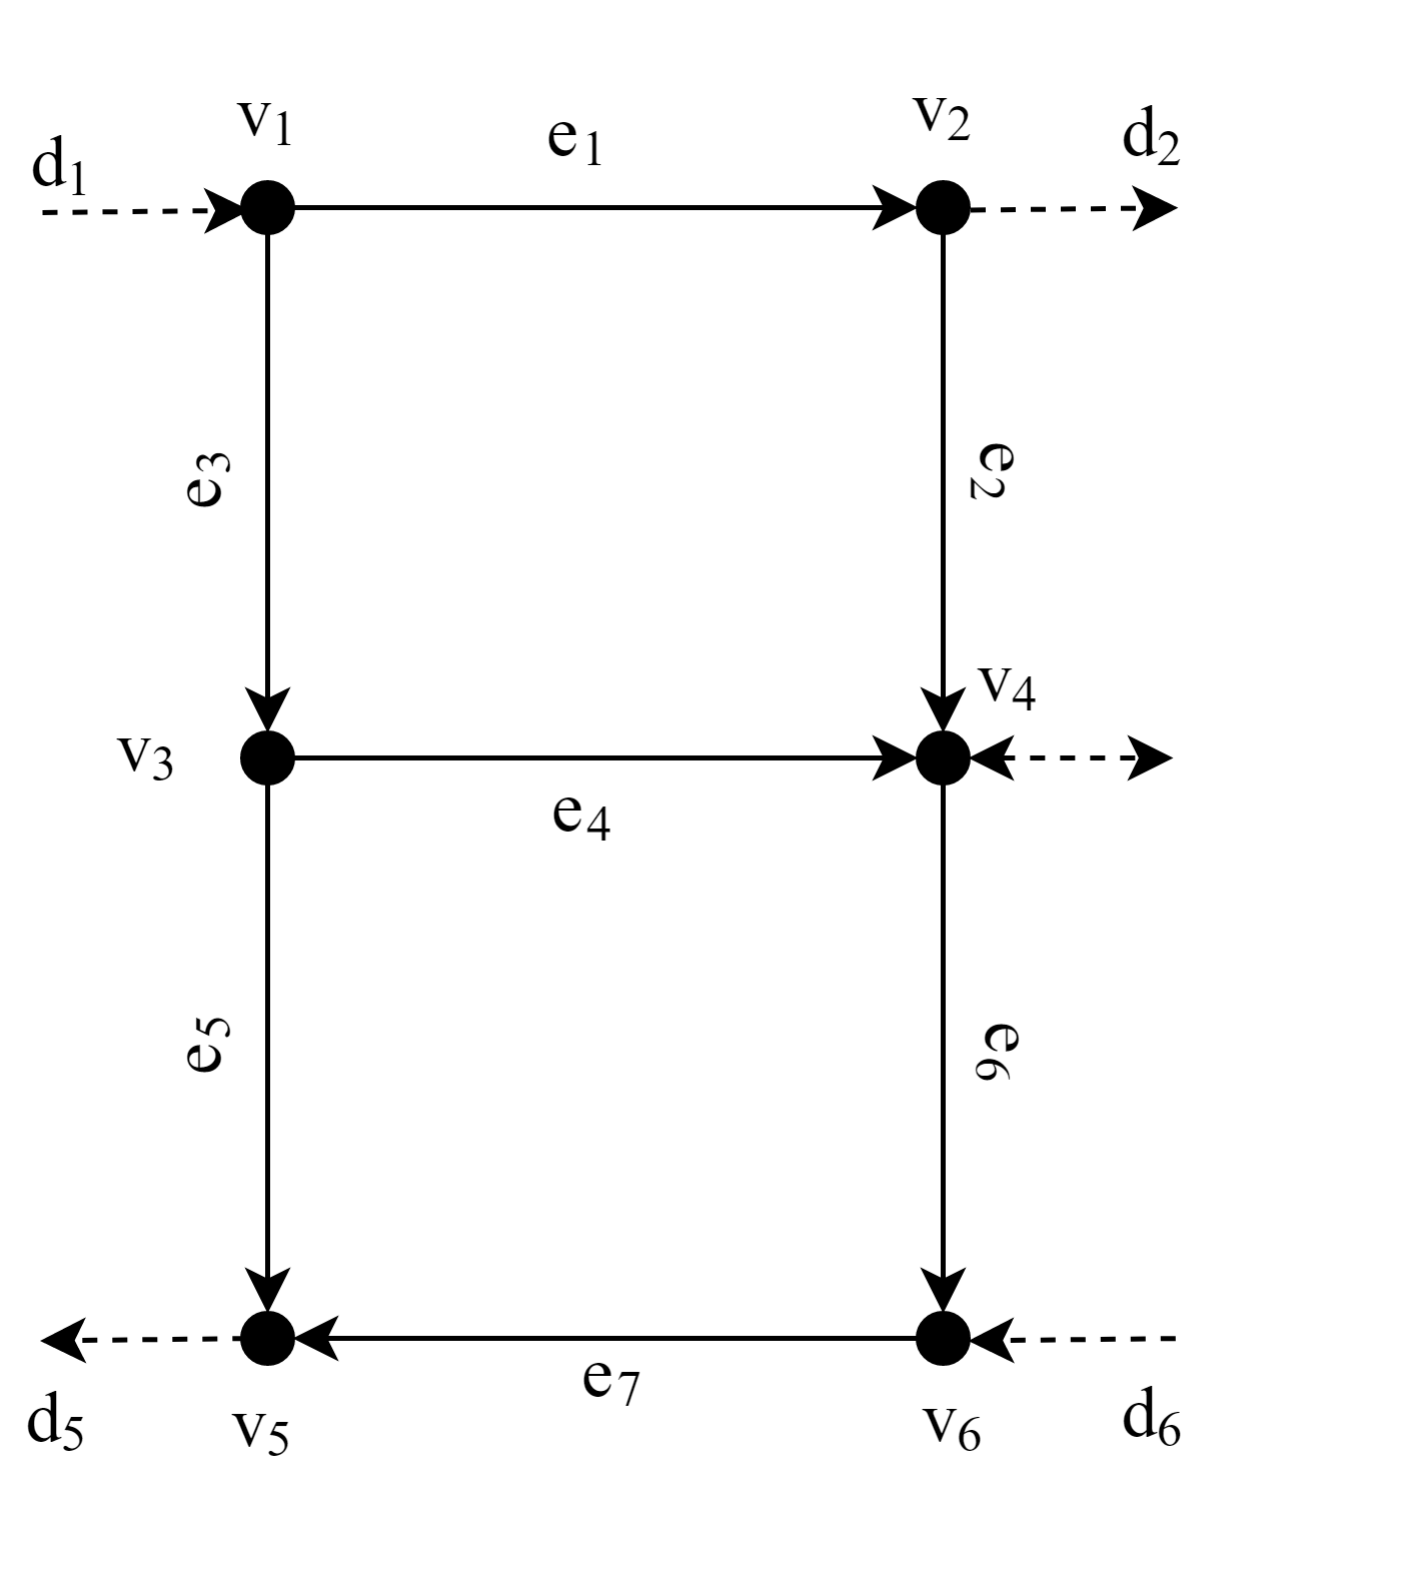
\includegraphics[width=0.5\textwidth]{Pictures/Graph.png}
	\caption{Graph of simplified WDN network \cite{Rathore930}}
	\label{fig:graph}
\end{figure}

When applying the rules shown above for the simplified graph model of the WDN the incident matrix in \cref{eq:H_simplified}.

\begin{equation}
	H = \begin{bmatrix}
		1 & 0 & 1 & 0 & 0 & 0 & 0\\
		-1 & 1 & 0 & 0 & 0 & 0 & 0\\
		0 & 0 & -1 & 1 & 1 & 0 & 0\\
		0 & -1 & 0 & -1 & 0 & 1 & 0\\
		0 & 0 & 0 & 0 & -1 &  0  & -1\\
		0 & 0 & 0 & 0 & 0 & -1 & 1
	\end{bmatrix}
	\label{eq:H_simplified}
\end{equation} %The incident matrix for system


The reduced incident matrix by taking an arbitrary vertex as a reference, and removing that vertex-row from \cref{eq:H_simplified}. We chose the $4^{th}$ vertex, which results in the following reduced incident matrix:
\begin{equation}
	\bar{H} = \begin{bmatrix}
		1 & 0 & 1 & 0 & 0 & 0 & 0\\
		-1 & 1 & 0 & 0 & 0 & 0 & 0\\
		0 & 0 & -1 & 1 & 1 & 0 & 0\\
		0 & 0 & 0 & 0 & -1 &  0  & -1\\
		0 & 0 & 0 & 0 & 0 & -1 & 1
	\end{bmatrix}
\end{equation}

Chords and edges of the spanning tree

\begin{equation} 
	\begin{split}
		E_{C} &= \{e_{1},e_{4}\}   \\ E_{T} &= \{e_2,e_3,e_5,e_6,e_7\}
	\end{split}
\end{equation}


\begin{equation}
	B = \begin{bmatrix}
		1 & 0 & 1 & -1 & -1 & 1 & 1\\
		0 & 1 & 0 & 0 & -1 & 1 & 1\\
	\end{bmatrix}
\end{equation}
\newpage

\subsection{Detailed system}
In this section we present a graph of the water distribution network.

\begin{figure}[h!]
	
	\centering
	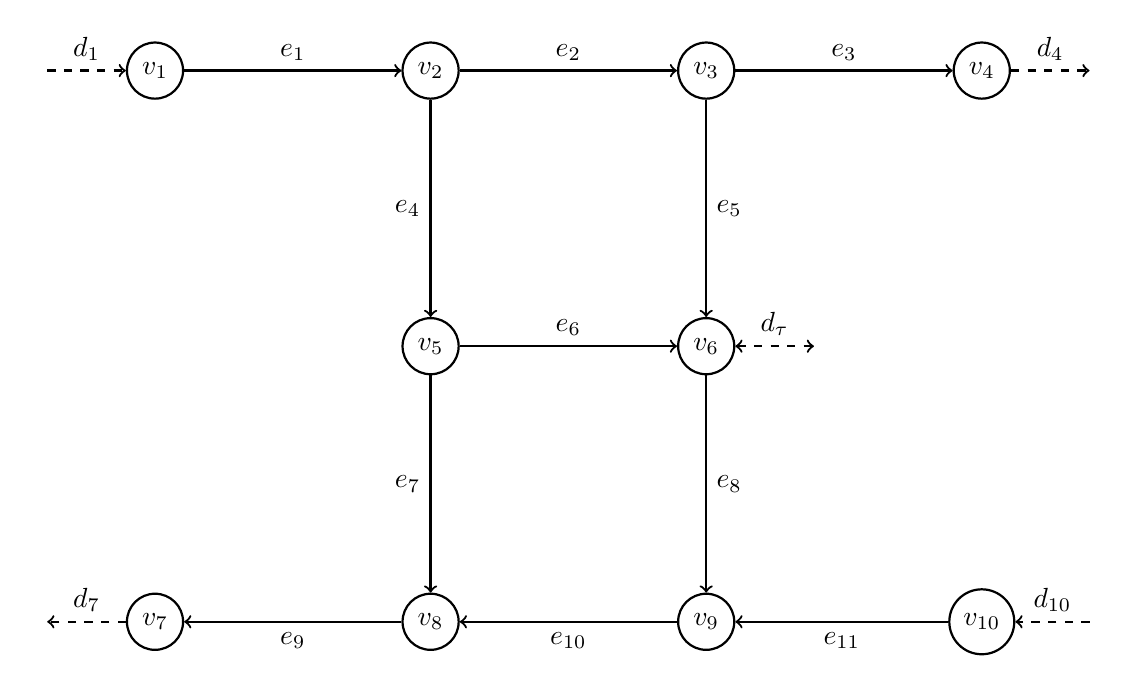
\begin{tikzpicture}[node distance=35mm,thick, main/.style = {draw, circle}] 
		\node (1)  {};
		\node[main] (2) [node distance={15mm},right of=1] {$v_1$}; 
		\node[main] (3) [right of=2] {$v_2$};
		\node[main] (4) [right of=3] {$ v_3 $};
		\node[main] (5) [right of=4] {$ v_4 $};
		\node (6) [node distance={15mm},right of=5] {};
		%Create 2 (3) nodes in middle part of graph
		\node[main] (7) [below of=3] {$ v_5 $};
		\node[main] (8) [below of=4] {$ v_6 $};
		\node (9) [node distance={15mm},right of=8] {};
		%Create 4 (6) nodes in bottom part of the graph
		\node[main] (10) [below of=7] {$v_8$}; 
		\node[main] (11) [left of=10] {$v_7$};
		\node (12) [node distance={15mm},left of=11] {};
		\node[main] (13) [right of=10] {$ v_9 $};
		\node[main] (14) [right of=13] {$ v_{10} $};
		\node (15) [node distance={15mm},right of=14] {};
		
		%Edges with direction
		\path [->] (2) edge node[above] {$e_1$} (3); %Edge v1 -> v2
		\path [->] (3) edge node[above] {$e_2$} (4); %Edge v2 -> v3
		\path [->] (4) edge node[above] {$e_3$} (5); %Edge v3 -> v4
		
		\path [->] (3) edge node[left] {$e_4$} (7); %Edge v2 -> v5
		\path [->] (4) edge node[right] {$e_5$} (8); %Edge v3 -> v6
		\path [->] (7) edge node[above] {$e_6$} (8); %Edge v5 -> v6
		
		\path [->] (7) edge node[left] {$e_7$} (10); %Edge v5 -> v8
		\path [->] (8) edge node[right] {$e_8$} (13); %Edge v6 -> v9
		
		\path [->] (10) edge node[below] {$e_9$} (11); %Edge v8 -> v7
		\path [->] (13) edge node[below] {$e_{10}$} (10); %Edge v9 -> v8
		\path [->] (14) edge node[below] {$e_{11}$} (13); %Edge v10 -> v9
		
		%External flows
		\draw[->,dashed,] (1) -- node[above] {$d_1$} (2); %Create d1
		\draw[->,dashed,] (5) -- node[above] {$d_4$} (6); %Create d4
		\draw[<->,dashed,] (8) -- node[above] {$d_\tau$} (9); %create d_tau
		\draw[->,dashed,] (11) -- node[above] {$d_7$} (12); %create d7
		\draw[->,dashed,] (15) -- node[above] {$d_{10}$} (14); %Create d10
		
	\end{tikzpicture} 
	\caption{Graph network of water distributed network}
\end{figure}
$ d_1 $ and $ d_{10} $ represent the waterflow into the system from the pumps, which are represented by edge $ e_1 $ and $ e_{11} $ respectively.
$ d_4 $ and $ d_7 $ represent the waterflow out of the system from the valves, which are represented by edge $ e_3 $ and $ e_9 $ respectively.
$ d_\tau $ represent the waterflow in an out of the tank.
The incident matrix for the graph on \cref{fig:WDNDetailed} is shown blow in \cref{eq:H_detailed}.
	
	\begin{equation}\label{eq:H_detailed}
		H = \kbordermatrix{
		& e_1 & e_2 & e_3   & e_4  & e_5 & e_6  & e_7  & e_8  & e_9  & e_{10}  & e_{11}  \\	
		v_1& 1 & 0 & 0   & 0  & 0  & 0  & 0  & 0  & 0  & 0  & 0 \\
		v_2& -1 & 1 & 0  & 1  & 0  & 0  & 0  & 0  & 0  & 0  & 0 \\
		v_3& 0 & -1 & 1  & 0  & 1  & 0  & 0  & 0  & 0  & 0  & 0 \\
		v_4& 0 & 0  & -1 & 0  & 0  & 0  & 0  & 0  & 0  & 0  & 0 \\
		v_5& 0 & 0  & 0  & -1 & 0  & 1  & 1  & 0  & 0  & 0  & 0 \\
		v_6&0 & 0  & 0  & 0  & -1 & -1 & 0  & 1  & 0  & 0  & 0 \\
		v_7& 0 & 0  & 0  & 0  & 0  & 0  & 0  & 0  & -1 & 0  & 0 \\
		v_8& 0 & 0  & 0  & 0  & 0  & 0  & -1 & 0  & 1  & -1 & 0 \\
		v_9& 0 & 0  & 0  & 0  & 0  & 0  & 0  & -1 & 0  & 1  & -1 \\
		v_{10}& 0 & 0  & 0  & 0  & 0  & 0  & 0  & 0  & 0  & 0  & 1 \\
	}
	\end{equation}	
	
The chords and the spanning tree is chosen from \cref{fig:WDNDetailed} \footnote{Note that you can obtain several spanning trees in this network, just by choosing different chords}
	
\begin{equation*} 
	\begin{split}
		E_{C} &= \{e_{2},e_{6}\}   \\ E_{T} &= \{e_1,e_3,e_4,e_5,e_7, e_8, e_9, e_{10} , e_{11}\}
	\end{split}
\end{equation*}	
	
	By choosing the xxx node as a reference, and removing it from the incident matrix we obtain:
	\begin{equation}
		\bar{H} = \kbordermatrix{
		& e_1 & e_2 & e_3   & e_4  & e_5 & e_6  & e_7  & e_8  & e_9  & e_{10}  & e_{11}  \\	
		v_1& 1 & 0 & 0   & 0  & 0  & 0  & 0  & 0  & 0  & 0  & 0 \\
		v_2& -1 & 1 & 0  & 1  & 0  & 0  & 0  & 0  & 0  & 0  & 0 \\
		v_3& 0 & -1 & 1  & 0  & 1  & 0  & 0  & 0  & 0  & 0  & 0 \\
		v_4& 0 & 0  & -1 & 0  & 0  & 0  & 0  & 0  & 0  & 0  & 0 \\
		v_5& 0 & 0  & 0  & -1 & 0  & 1  & 1  & 0  & 0  & 0  & 0 \\
		v_7& 0 & 0  & 0  & 0  & 0  & 0  & 0  & 0  & -1 & 0  & 0 \\
		v_8& 0 & 0  & 0  & 0  & 0  & 0  & -1 & 0  & 1  & -1 & 0 \\
		v_9& 0 & 0  & 0  & 0  & 0  & 0  & 0  & -1 & 0  & 1  & -1 \\
		v_{10}& 0 & 0  & 0  & 0  & 0  & 0  & 0  & 0  & 0  & 0  & 1 \\
		}
	\end{equation}
	
Furthermore we can define the open-node matrix $F$ and tank matrix $G$:
	
	\begin{equation}\label{eq:ONandTankMatrix}
		F = \kbordermatrix{
			&d_{f_1}&d_{f_2}&d_{f_3}&d_{f_4}\\
		d_1	& 1 & 0 & 0 & 0\\
		d_2	& 0 & 0 & 0 & 0\\
		d_3 & 0 & 0 & 0 & 0\\
		d_4 & 0 & 1 & 0 & 0\\
		d_5 & 0 & 0 & 0 & 0\\
		d_6 & 0 & 0 & 0 & 0\\
		d_7 & 0 & 0 & 1 & 0\\
		d_8 & 0 & 0 & 0 & 0\\
		d_9 & 0 & 0 & 0 & 0\\
		d_{10}& 0 & 0 & 0 & 1 \\
			},
	\qquad
		G = \kbordermatrix{
			&d_{\tau_1}\\
			d_1& 0\\
			d_2& 0\\
			d_3& 0\\
			d_4& 0\\
			d_5& 0\\
			d_6& 1\\
			d_7& 0\\
			d_8& 0\\
			d_9& 0\\
			d_{10}& 0 \\
			}
	\end{equation}

with their reference-respective equivalents given by:

\begin{equation}\label{eq:FbarGbar}
	\bar{F} = F \setminus F_{6\star} \wedge \bar{G} = G \setminus G_{6\star}
\end{equation}

where the notation $X_{6\star}$ denotes the entire 6th row\footnote{Correspondingly, $X_{\star6}$ would denote the entire 6th column} of the matrix $X$ and $\setminus$ is the set relative complement operator. These matrices map demands at their respective nodes into the vector of total demands in the system $d \vee \bar{d}$.

\subsection{Implementation of Detailed system}

\begin{figure}[h!]
	
	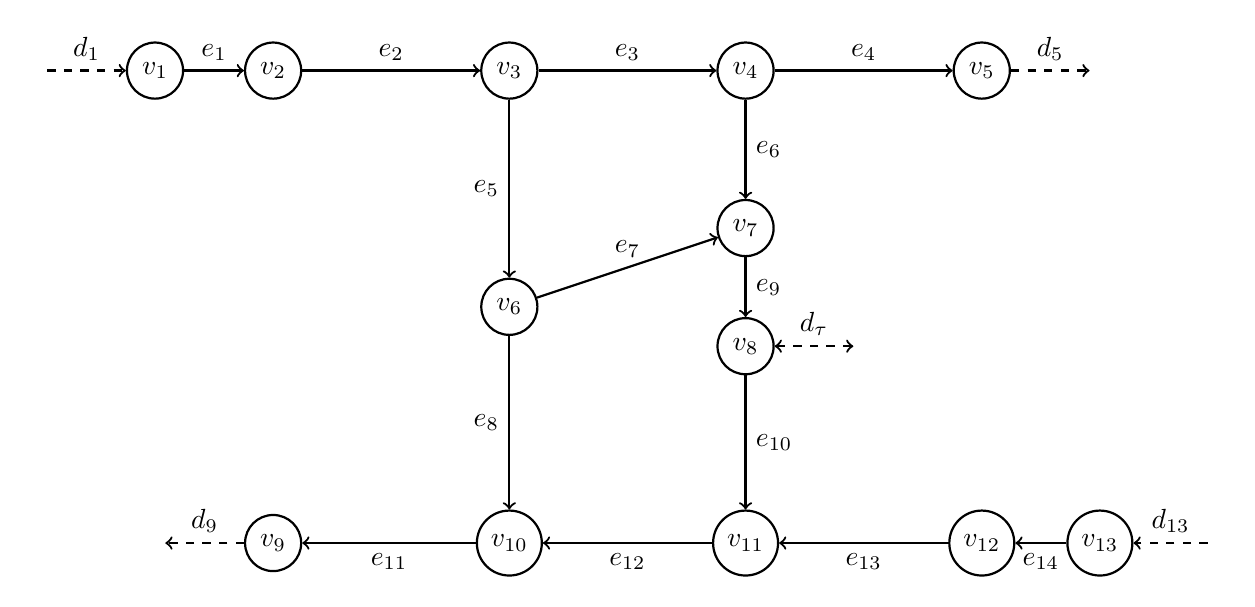
\begin{tikzpicture}[node distance=30mm, thick, main/.style = {draw,circle}] 
		\node (1)  {};
		\node[main] (2) [node distance={15mm},right of=1] {$v_1$}; 
		\node[main] (3) [node distance={1.5cm},right of=2] {$v_2$};
		\node[main] (4) [right of=3] {$v_3$};
		\node[main] (5) [right of=4] {$v_4$};
		\node[main] (6) [right of=5] {$v_5$};
		\node (7) [node distance={15mm},right of=6] {};
		%Create 3 (4) nodes in middle part of graph
		\node[main] (8) [below of=4] {$ v_6 $};
		\node[main] (9) [node distance={20mm},below of=5] {$ v_7 $};
		\node[main] (11) [node distance={15mm},below of=9] {$ v_8 $};
		\node (10) [node distance={15mm},right of=11] {};
		%First 5 (7) nodes in bottom part of graph
		\node[main] (12) [below of=8] {$ v_{10} $};
		\node[main] (13) [left of=12] {$ v_9 $};
		\node(14) [node distance={15mm},left of=13] {};
		\node[main] (15) [right of=12] {$ v_{11} $};
		\node[main] (16) [right of=15] {$ v_{12} $};
		\node[main] (17) [node distance={1.5cm},right of=16] {$ v_{13} $};
		\node(18) [node distance={15mm},right of=17] {};
		
		%Edges with direction
		\path [->] (2) edge node[above] {$e_{1}$} (3); 	%Edge v1 -> v2
		\path [->] (3) edge node[above] {$e_{2}$} (4); 	%Edge v2 -> v3
		\path [->] (4) edge node[above] {$e_{3}$} (5); 	%Edge v3 -> v4
		\path [->] (5) edge node[above] {$e_{4}$} (6); 	%Edge v4 -> v5
		
		\path [->] (4) edge node[left] {$e_{5}$} (8); 	%Edge v3 -> v6
		\path [->] (5) edge node[right] {$e_{6}$} (9); 	%Edge v4 -> v7
		\path [->] (8) edge node[above] {$e_{7}$} (9); 	%Edge v6 -> v7
		\path [->] (8) edge node[left] {$e_{8}$} (12); 	%Edge v6 -> v10
		\path [->] (9) edge node[right] {$e_{9}$} (11); 	%Edge v7 -> v8
		\path [->] (11) edge node[right] {$e_{10}$} (15);	 %Edge v8 -> v11
		
		
		\path [->] (12) edge node[below] {$e_{11}$} (13); %Edge v10 -> v9
		\path [->] (15) edge node[below] {$e_{12}$} (12); %Edge v11 -> v10
		\path [->] (16) edge node[below] {$e_{13}$} (15); %Edge v12 -> v11
		\path [->] (17) edge node[below] {$e_{14}$} (16); %Edge v13 -> v12
		
		%External flows
		\draw[->,dashed,] (1) -- node[above] {$d_1$} (2); %Create d1
		\draw[->,dashed,] (6) -- node[above] {$d_5$} (7); %Create d5
		\draw[->,dashed,] (13) -- node[above] {$d_9$} (14); %Create d13
		\draw[->,dashed,] (18) -- node[above] {$d_{13}$} (17); %Create d13
		\draw[<->,dashed,] (10) -- node[above] {$d_\tau$} (11); %Create d_tau
	\end{tikzpicture} 
	\caption{Graph network of implemented water distributed network}
\end{figure}

The H matrix:

	\begin{equation}\label{eq:labH}
	H = \kbordermatrix{
		&e_1&e_2&e_3&e_4&e_5&e_6&e_7&e_8&e_9&e_{10}&e_{11}&e_{12}&e_{13}&e_{14} \\	
v_{1}&	1	&0	& 0 & 0 & 0	& 0 & 0	& 0	& 0	& 0 & 0	& 0	& 0	& 0 \\
v_{2}&	-1	& 1 & 0	& 0	& 0	& 0	& 0	& 0	& 0	& 0 & 0	& 0	& 0 & 0 \\
v_{3}&	0	& -1& 1	& 0 & 1 & 0 & 0 & 0 & 0 & 0 & 0	& 0 & 0 & 0 \\
v_{4}&	0	& 0 &-1 & 1 & 0 & 1 & 0 & 0 & 0	& 0	& 0	& 0	& 0	& 0 \\
v_{5}&	0	& 0 & 0	& -1& 0	& 0	& 0	& 0	& 0	& 0	& 0	& 0	& 0	& 0 \\
v_{6}&	0	& 0	& 0	& 0	& -1& 0	& 1	& 1	& 0	& 0 & 0	& 0	& 0 & 0 \\
v_{7}&	0	& 0	& 0	& 0	& 0 & -1& -1& 0	& 1 & 0 & 0	& 0	& 0	& 0 \\
v_{8}&	0	& 0	& 0	& 0	& 0 & 0 & 0 & 0	& -1& 1 & 0	& 0	& 0	& 0 \\
v_{9}&	0	& 0	& 0	& 0	& 0 & 0 & 0 & 0	& 0 & 0 & -1& 0	& 0	& 0 \\
v_{10}&	0	& 0	& 0	& 0	& 0 & 0 & 0 & -1& 0 & 0 & 1 & -1& 0	& 0 \\
v_{11}&	0	& 0	& 0	& 0	& 0 & 0 & 0 & 0 & 0 & -1& 0 & 1 & -1& 0 \\
v_{12}&	0	& 0	& 0	& 0	& 0 & 0	& 0 & 0 & 0 & 0 & 0 & 0 & 1	& -1\\
v_{13}&	0	& 0	& 0	& 0	& 0 & 0	& 0 & 0 & 0 & 0 & 0 & 0 & 0	& 1    
	} 
\end{equation}	


The reduced incident matrix $ \bar{H} $ for the system given by \cref{eq:labH} is obtained by choosing the node 13 as reference:

	\begin{equation}\label{eq:H_detailed}
	\bar{H} = \kbordermatrix{
		&e_1&e_2&e_3&e_4&e_5&e_6&e_7&e_8&e_9&e_{10}&e_{11}&e_{12}&e_{13}&e_{14} \\	
		v_{1}&	1	&0	& 0 & 0 & 0	& 0 & 0	& 0	& 0	& 0 & 0	& 0	& 0	& 0 \\
		v_{2}&	-1	& 1 & 0	& 0	& 0	& 0	& 0	& 0	& 0	& 0 & 0	& 0	& 0 & 0 \\
		v_{3}&	0	& -1& 1	& 0 & 1 & 0 & 0 & 0 & 0 & 0 & 0	& 0 & 0 & 0 \\
		v_{4}&	0	& 0 &-1 & 1 & 0 & 1 & 0 & 0 & 0	& 0	& 0	& 0	& 0	& 0 \\
		v_{5}&	0	& 0 & 0	& -1& 0	& 0	& 0	& 0	& 0	& 0	& 0	& 0	& 0	& 0 \\
		v_{6}&	0	& 0	& 0	& 0	& -1& 0	& 1	& 1	& 0	& 0 & 0	& 0	& 0 & 0 \\
		v_{7}&	0	& 0	& 0	& 0	& 0 & -1& -1& 0	& 1 & 0 & 0	& 0	& 0	& 0 \\
		v_{8}&	0	& 0	& 0	& 0	& 0 & 0 & 0 & 0	& -1& 1 & 0	& 0	& 0	& 0 \\
		v_{9}&	0	& 0	& 0	& 0	& 0 & 0 & 0 & 0	& 0 & 0 & -1& 0	& 0	& 0 \\
		v_{10}&	0	& 0	& 0	& 0	& 0 & 0 & 0 & -1& 0 & 0 & 1 & -1& 0	& 0 \\
		v_{11}&	0	& 0	& 0	& 0	& 0 & 0 & 0 & 0 & 0 & -1& 0 & 1 & -1& 0 \\
		v_{12}&	0	& 0	& 0	& 0	& 0 & 0	& 0 & 0 & 0 & 0 & 0 & 0 & 1	& -1\\
		%v_{13}&	0	& 0	& 0	& 0	& 0 & 0	& 0 & 0 & 0 & 0 & 0 & 0 & 0	& 1    
	}
\end{equation}	
The B matrix (not even started):

$ B = \begin{bmatrix}
	1	& 0 	& 0 	& 0 	& 0 	& 0 	& 0 	& 0 	& 0 	& 0 	& 0 	& 0 \\
	-1	& 1 	& 0 	& 0 	& 0 	& 0 	& 0 	& 0 	& 0 	& 0 	& 0 	& 0 \\
\end{bmatrix}  $



\clearpage

\section{WDN Component Models}\label{sec:ComponentModels}

All components (eg. pipes, valves and pumps) can be described by two variables, namely the flow through the component and the differential pressure across the component:
\begin{equation}
\begin{bmatrix} \Delta{p_{k}} \\ q_{k} \end{bmatrix} = 
\begin{bmatrix} p_{i} - p_{j} \\ q_{k} \end{bmatrix}    
\end{equation}

The following section will examine these two variables for pipes, valves and pumps. We source the equations from \cite{MathiasBjarni2015}.

\subsection{Pipe Model}\label{subsec:PipeModel}
The differential pressure across a pipe can be modelled as follows:
\begin{equation}
    \mathrm{\Delta{p_{k}}} = J_{k}\cdot\dot{q_{k}}+\mathrm{\lambda_{k}}(q_{k})-\mathrm{\Delta{z_{k}}}
    \label{eq:Delta_p_pipe}
\end{equation}


	\begin{center}
		\begin{tabular}{l p{10cm} l}
			
			$\Delta{p_{k}}$ & The differential pressure across the $k$th component & [\si{Pa}]\\ 
		  	${J_{k}}$ & The mass inertia of the water in the $k$th pipe & [\si{kg}/\si{m^{4}}] \\
		  	$q_{k}$ & is the flow of water trough the $k$th pipe & [{\si{\meter\cubed}/\si{s}}] \\
		  	$\mathrm{\lambda_{k}}(q_{k})$ & is the drop in pressure due to friction in the $k$th pipe & [\si{Pa}] \\
		  	$\mathrm{\Delta{z_{k}}}$ & is the drop in pressure due to geodesic level & [\si{Pa}]\\
			\end{tabular}
	\end{center}

The mass inertia of water can be describes as follows:
\begin{equation}
	J= \frac{L\cdot \rho}{A}
\end{equation}

	\begin{center}
		\begin{tabular}{l p{10cm} l}
			$L$ & is the length of the pipe & [\si{m}]\\
			$\rho$ & is the density of water & [\si{kg}/\si{m\cubed}]\\  
			$A$ & is the cross sectional area of water & [\si{m\squared}]\\ 
		\end{tabular}
	\end{center}
The cross-sectional area of the pipe is assumed to be constant along the pipe.

The causes of flow friction $\mathrm{\lambda_{k}}(q_{k})$ are surface resistance $h_{f}$ and form resistance $h_{m}$. The surface resistance can be described with the Darcy-Weisbach equation:

\begin{equation}
	h_{f} = f \cdot \frac{8\cdot L\cdot q^{2}}{\pi^{2}\cdot g \cdot D^{5}}
\end{equation} 

\begin{center}
	\begin{tabular}{l p{10cm} l}
		$h_{f}$ & is the head loss from surface resistance & [\si{m}]\\
		$f$ & is the pipe friction factor & [$\cdot$]\\
		$D$ & is the pipe diameter & [\si{m}]\\
		$g$ & is the gravitational constant & [\si{m}/\si{s\squared}]\\
	\end{tabular}
\end{center}
Under the assumption of turbulent flow $f$ is given by:
\begin{equation}
	f=1.325\cdot \Bigg(ln\Big(\frac{\epsilon}{3.7 \cdot D}+\frac{5.74}{R^{0.9}}\Big)\Bigg)^{-2}
\end{equation}

\begin{center}
	\begin{tabular}{l p{8cm} l}
		$\epsilon$ & average roughness height in the pipe & [\si{m}]\\
		$R$ &  is Reynolds number - for turbulent flow $R \geq 4000$ & [$\cdot$]\\
	\end{tabular}
\end{center}

The form resistance is given by the following:
\begin{equation}
	h_{m}=k_{f}\cdot \frac{8\cdot q^{2}}{\pi^{2}\cdot g \cdot D^{4}}
\end{equation}

\begin{center}
	\begin{tabular}{l p{8cm} l}
		$h_{m}$ & is the head loss from form resistances & [\si{m}]\\
		$k_{f}$ &  is coefficient form loss & [$\cdot$]\\
	\end{tabular}
\end{center}

The drop in pressure due to geodesic level difference:
\begin{equation}
	\Delta{z_{k}} = \rho \cdot g \cdot \Delta{h_{k}}
\end{equation}

\begin{center}
	\begin{tabular}{l p{8cm} l}
		$\Delta{h_{k}}$ &  is the level difference across the terminals of the $k$th pipe & [\si{m}]\\
	\end{tabular}
\end{center}

Having explained all the components of \eqref{eq:Delta_p_pipe} a complete expression can now be formulated; we take advantage of the fact that resistance losses are expressed in terms of head, and can be expressed in terms of pressure by multiplying by $\rho$ and g. \begin{equation}
	p = \rho \cdot g \cdot h  
\end{equation}

Meaning that the head losses can be expressed in terms of pressure by the following:

\begin{equation}
\lambda_{k}(q_{k})  =	\Big(f \cdot \frac{8\cdot L\cdot q^{2}}{\pi^{2}\cdot g \cdot D^{5}} + k_{f}\cdot \frac{8\cdot q^{2}}{\pi^{2}\cdot g \cdot D^{4}}\Big)\cdot g \cdot \rho
\end{equation}

Inserting and reducing into \cref{eq:Delta_p_pipe}

\begin{equation}
	\Delta{p_{k}} = \frac{L\cdot \rho}{A}\cdot \dot{q_{k}}
	+\Big(f \cdot \frac{8\cdot L\cdot \rho}{\pi^{2} \cdot D^{5}} + k_{f}\cdot \frac{8\cdot \rho}{\pi^{2} \cdot D^{4}}\Big)\cdot |q_{k}|\cdot q_{k} 
	- \rho \cdot g \cdot \Delta{h_{k}} = \mathcal{J}\dot{q} + \lambda(q) + \Delta z
\end{equation}

The absolute value of one of the flow component in $q^{2}$ is taken to preserve the flow direction.


\subsection{Valve Model}\label{subsec:ValveModel}

While the head loss of a valve \textit{can} be explained in terms of its form resistance, as we have done previously in \cref{subsec:PipeModel}, it is generally impractical to determine the form loss coefficient $k_f$ for valves. Instead, an expression for the head loss can be derived - typically by the manufacturer - via a conductivity function $K_{valve}(OD)$.

\smallskip

Recalling that the pressure drop across a valve is proportional to its squared flow, we may express that:

\begin{equation}\label{eq:HydrodynamicRatio}
	\frac{\Delta p_1}{q_1^2} = \frac{\Delta p_2}{q_2^2} \Leftrightarrow 
	\frac{\Delta p_1}{\Delta p_2} = \frac{q_1^2}{q_2^2}
	\Leftrightarrow
	q_1 = q_2\cdot\sqrt{\frac{\Delta p_1}{\Delta p_2}}
\end{equation}

We then express the conductivity function $K_{valve}(OD)$, by convention, as corresponding to the flow $q_n$ at a given opening degree that produces exactly a pressure differential of 1 bar, i.e.:

\begin{equation}\label{eq:Kvalve}
	q = q_n(OD)\cdot\sqrt{\frac{\Delta p_1}{1}} = K_{valve}(OD)\cdot\sqrt{\Delta p_1}
\end{equation}

We can then express the pressure differential across the valve for a given flow as:

\begin{equation}\label{eq:ValvePressure}
	 q = K_{valve}(OD)\cdot\sqrt{\Delta p_1}
	 \Leftrightarrow
	 \Delta p_1 = \frac{1}{K_{valve}(OD)^2} \cdot |q|\cdot q = \mu(q,OD)
\end{equation}

where $q^2 \equiv |q|\cdot q$ is introduced to preserve the directionality of flow. Note that \cref{eq:ValvePressure} implies the pressure differential across the pipe varies with both flow rate \textit{and} opening degree.

\smallskip

$K_{valve}(OD)$ may take a variety of forms, but is typically either linear, equal-percentage, or quick-opening.

\subsection{Pump Model}\label{subsec:PumpModel}

The pressure differential across a centrifugal pump, such as the pumps used in this project, is a multivariable function that can generally be approximated by a polynomial expression of the form:

\begin{equation}\label{eq:PumpPressure}
	\Delta p =   a_0\cdot \omega^2 +  a_1\cdot \omega \cdot q -a_2\cdot |q|\cdot q
\end{equation}

where $[a_0,a_1,a_2]$ is a tuple of coefficients that describe the pump's characteristic curve, $q$ is the flow rate through the pump, and $\omega$ is the rotational velocity of the pump.

\subsection{Elevated Water Reservoir Model}

In this section we will develop a hydraulic model of an elevated fluid reservoir, also known as a tank.
Under assumption that the cross-sectional area of the tank is constant along its height axis, the pressure at the bottom of the tank is proportional to the fluid level in the tank:

\begin{equation} \label{eq:p prop zeta}
	p_\tau \propto \zeta
\end{equation}

The volumetric rate of change is equal to the flow in and out of the tank:

\begin{equation} \label{eq:vdot = dt}
	\dot{V} = d_\tau
\end{equation}

Logically, the rate of fluid level change is proportional to the volumetric rate of change:  
 
 \begin{equation} \label{eq:zeta prop dt}
	\dot{\zeta} \propto \dot{V} \Leftrightarrow \dot{\zeta} \propto d_\tau
\end{equation} 

From above it can be concluded that the rate of change of pressure is proportional to flow in and out of the tank:

\begin{equation} \label{eq:dotp prop dt}
	\dot{p}_{\tau} \propto d_\tau 
\end{equation}

Defining the proportionality constant $\tau$ and taking flow out of the tank as positive:

\begin{equation} \label{eq:dpTank}
	\dot{p}_{\tau}=-\tau \cdot d_{\tau} 
\end{equation} 

\begin{center}
	\begin{tabular}{l p{10cm} l}
		$p_\tau$ & is the pressure at the node connected to the bottom of the tank & [\si{Pa}]\\
		$\tau$ & is the tank parameter which depends on the cross sectional area of the tank & [\si{Pa}/\si{m\cubed}]\\
		$d_\tau$ & is the water flow in and out of the tank. If $q > 0$ water is flowing out of the tank, if $q < 0$ water is flowing into the tank. & [\si{m\cubed}/\si{s}] 
		\end{tabular}
\end{center}

The tank parameter is given by:
\begin{equation}\label{eq:TankParameter}
\tau = \rho \cdot g \frac{1}{A}
\end{equation}
 


\clearpage

\section{WDN System Model}\label{sec:SystemModel}

In this section we will develop the model of the water distribution network, based on the graph theory presented in \cref{sec:GraphTheory}.

\subsection{Assumptions and Lemmas}\label{subsec:AsssumAndLemmas}

In modelling the dynamics of an open hydraulic network, we will make a few basic physical assumptions. Assuming a network with topology described by the incidence matrix $H$ and fundamental loop matrix $B$, subject to the vector of \textit{nodal} flows $d \in \mathbb{R}^n$, and containing the \textit{edge} flows $q \in \mathbb{R}^m$. We will assume that this system is obeys Kirchoff's Nodal Law (KNL), i.e. that:

\begin{equation}\label{eq:KirchNodeLaw}
	H\cdot q = d
\end{equation} 

We also assume that the system obeys Kirchoff's Mesh Law (KML), i.e.:

\begin{equation}\label{eq:KirchMeshLaw}
	B\Delta p = B H^T p = 0 \wedge B\Delta h = B H^T h = 0
\end{equation}

Furthermore, we assume that the system is conservative with respect to mass, which implies that there can at most be $n-1$ independent nodal demands, i.e.:

\begin{equation}\label{eq:MassConservation}
	d_n = -\sum_{i=1}^{n-1}d_i
\end{equation}

We will also define a set of graph-theoretical lemmas for convenience, referring to \cite{Jensen} for proof of both:

\begin{lemma}\label{lem:TreePartitionLemma}
	Let $H_T$ be the incidence matrix partition corresponding to the spanning tree of the graph described by $H$, and let $\bar{H}_T$ be its equivalent with respect to the reduced incidence matrix $\bar{H}$. $\bar{H}_T$ is invertible since a tree is a connected graph with $n-1$ edges \cite{Deo}, and the following holds
	
	\begin{equation}\label{eq:TreePartitionLemma}
		H_T\cdot\bar{H}_T^{-1} = \begin{bmatrix} I_{n-1} \\ \mathbf{1}^T	\end{bmatrix}
	\end{equation}

where $\mathbf{1}$ is a vector of ones and $I_{n-1} \in \mathbb{R}^{n-1 \times n-1}$ is an identity matrix.
\end{lemma}

\begin{lemma}\label{lem:EdgeFlowDecomposition}
	Let $q \in \mathbb{R}^m$ be the edge flows of a graph with reduced incidence matrix $\bar{H}$ and $n$ nodes. Denote its spanning tree by $T$, let $q_c \in \mathbb{R}^c, \ c = m-n+1$ be the graph's chordal flows, and denote the tree partition of the reduced incidence matrix $\bar{H}_T$. Finally, let $B$ be the graph's fundamental loop matrix, and define $\bar{d} \in \mathbb{R}^{n-1}$ as the vector of non-reference nodal flows. Then the following is true:
	
	\begin{equation}\label{eq:EdgeFlowDecomposition}
		q = B^T\cdot q_c +
		\begin{bmatrix}
			0_{c \times n-1} \\ \bar{H}_T^{-1} 
		\end{bmatrix}
		\cdot \bar{d}
	\end{equation}
\end{lemma}

We are now ready to start modelling the system.

\subsection{Modelling an Open Hydraulic Network with an Elevated Reservoir}\label{subsec:ModelWithTank}

We assume a network topology with $n$ nodes and $m$ edges, of which $e$ nodes are open to the atmosphere. By definition, water can only flow in and out of the network at nodes which are open to the atmosphere, implying that the nodal demand at the $d-e$ non-open nodes is zero at all times. Assuming now that an open node has been chosen as the reference node, the vector of all independent flows $\bar{d}$ can be obtained from the non-zero flows $d_f \in \mathbb{R}^{e-1}$ by:

\begin{equation}\label{eq:IndependentFlows}
	\bar{d} = F\cdot d_f, \ F = \begin{bmatrix}
		I_{e-1} \\ 0
	\end{bmatrix}
\end{equation}

with the remaining nodal demand at the reference node comprising the dependent flow. The edge flows can then be expressed, using \cref{lem:EdgeFlowDecomposition} to re-write KNL \cref{eq:KirchNodeLaw}, as:

\begin{equation}\label{eq:EdgeFlows}
	q = B^T\cdot q_C +
	\begin{bmatrix} 0 \\ \bar{H}_T^{-1} \end{bmatrix} \cdot F \cdot d_f
\end{equation}

We can modify this to account for tanks by introducing an additional vector of non-zero demand nodes that is \textit{not} open to the atmosphere, denoting it $d_{\tau} \in \mathbb{R}^{\tau}$. We can then restate \cref{eq:IndependentFlows} as:

\begin{equation}\label{eq:IndependentFlowsWithTank}
	\bar{d} = F\cdot d_f + G \cdot d_{\tau}, 
	\ F = \begin{bmatrix}
		I_{e-1} \\ 0
	\end{bmatrix} 
	\wedge 
	G = \begin{bmatrix}
	0 \\ I_{\tau}
	\end{bmatrix}
\end{equation}

subsequently allowing \cref{eq:EdgeFlows} to be restated as:

\begin{equation}\label{eq:EdgeFlowsWithTank}
	q = B^T\cdot q_C +
	\begin{bmatrix} 0 \\ \bar{H}_T^{-1} \end{bmatrix} (F \cdot d_f + G \cdot d_{\tau})
\end{equation}

We can now state the pressure drop across each edge in the network as:

\begin{equation}\label{eq:PressureFunction}
	\Delta p = \mathcal{J}\dot{q} + \lambda(q) + \mu(q) + \alpha(q) -\Delta h
\end{equation}

where $\mathcal{J}, \lambda, \mu, \alpha$ are as defined in \cref{sec:ComponentModels}\footnote{Note that we have omitted the secondary variables $OD,\omega$ for convenience.} and $q$ is the vector of edge flows. We now invoke KML as per \cref{eq:KirchMeshLaw} on \cref{eq:PressureFunction}, obtaining:

\begin{equation}\label{eq:PressureFunctionKirch}
	\begin{split}
			0 &= B\mathcal{J}\dot{q} + B(\lambda(q) + \mu(q) + \alpha(q)) -B\Delta h \\
			&= B\mathcal{J}\dot{q} + B(\lambda(q) + \mu(q) + \alpha(q)) \\
			&\Rightarrow \\
			B\mathcal{J}\dot{q} &= -B(\lambda(q) + \mu(q) + \alpha(q))
	\end{split}
\end{equation}

We can then invoke KNL on the left-hand side of \cref{eq:PressureFunctionKirch}, resulting in:

\begin{equation}\label{eq:PressureFunctionKirchKNL}
	B\mathcal{J}B^T\dot{q_C} + B \mathcal{J} 
	\begin{bmatrix} 0 \\ \bar{H}_T^{-1} \end{bmatrix} \cdot (F \cdot \dot{d_f} + G \cdot \dot{d_{\tau}})
	= -B(\lambda(q) + \mu(q) + \alpha(q))
\end{equation}

We now develop this expression further via the definition of $B$ in \cref{eq:LoopMatrix} and via a chord/tree-partition of $\mathcal{J}$ such that:

\begin{equation}\label{eq:PressureFunctionKirchJPartitions}
	B\mathcal{J}B^T\dot{q_C} + 
	\begin{bmatrix}		I_C & -\bar{H}_C^T\bar{H}_T^{-T}	\end{bmatrix} 
	\begin{bmatrix}		\mathcal{J}_C & 0 \\ 0 & \mathcal{J}_T	\end{bmatrix} 
	\begin{bmatrix} 0 \\ \bar{H}_T^{-1} \end{bmatrix} \cdot (F \cdot \dot{d_f} + G \cdot \dot{d_{\tau}})
	= -B(\lambda(q) + \mu(q) + \alpha(q))
\end{equation}

This simplifies to:

\begin{equation}\label{eq:PressureFunctionKirchJPartitionsSimp} % KEKW
	B\mathcal{J}B^T\dot{q_C} 
	-\bar{H}_C^T\bar{H}_T^{-T}\mathcal{J}_T\bar{H}_T^{-1} F \dot{d_f} 
	-\bar{H}_C^T\bar{H}_T^{-T}\mathcal{J}_T\bar{H}_T^{-1} G \dot{d_{\tau}}
	= -B(\lambda(q) + \mu(q) + \alpha(q))
\end{equation}

We now recall that we have chosen a reference node that is open to atmosphere at $p_{ref} = p_0$, and that $\Delta p$ can be rewritten as: 

\begin{equation}\label{eq:DeltaPPartition}
	\Delta p =
	\begin{bmatrix}		\Delta p_C \\ \Delta p_T	\end{bmatrix} = 
	\begin{bmatrix}		H_C^T \\ H_T^T	\end{bmatrix} p
\end{equation}

It is then, given that an arbitrary node can be reached by pathing solely through the spanning tree, axiomatically true per KML that:

\begin{equation}\label{eq:RelativePressureKML}
	H_T^T p = 
	\bar{H}_T^T \begin{bmatrix} \bar{p} \\ p_0	\end{bmatrix} =
	\mathcal{J}_T\dot{q}_T + (\lambda_T(q_T)+\mu_T(q_T) + \alpha_T(q_T)) - 
	\bar{H}_T^T \begin{bmatrix} \bar{h} \\ h_0	\end{bmatrix}
\end{equation}

We now exploit that:

\begin{equation}\label{eq:TreeLemmaRewrite}
	H_T\cdot\bar{H}_T^{-1} = \bar{H}_T^{-T}H_T^T 
\end{equation}

which allows us to rewrite \cref{eq:RelativePressureKML} by left-multiplying every term with $\bar{H}_T^{-T}$ and exploiting \cref{lem:TreePartitionLemma}:

\begin{equation}\label{eq:RelativePressureKMLWithLemma}
	\bar{p} - \mathbf{1}p_0 =
	\bar{H}_T^{-T}\mathcal{J}_T\dot{q}_T + \bar{H}_T^{-T}(\lambda_T(q_T)+\mu_T(q_T) + \alpha_T(q_T)) - 
	(\bar{h} - \mathbf{1}h_0)
\end{equation}

Recalling that $F$ extracts the open nodes from the non-reference nodes, we can then express the following:

\begin{equation}\label{eq:RelativePressureLemmaAtmospheric}
	0 = F^T(\bar{p} - \mathbf{1}p_0) =
	F^T\Big(\bar{H}_T^{-T}\mathcal{J}_T\dot{q}_T + \bar{H}_T^{-T}(\lambda_T(q_T)+\mu_T(q_T) + \alpha_T(q_T))\Big) - 
	F^T(\bar{h} - \mathbf{1}h_0)
\end{equation}

which implies that: 

\begin{equation}\label{eq:RelativePressureLemmaDiffEqForm}
	F^T\bar{H}_T^{-T}\mathcal{J}_T\dot{q}_T = - F^T\Big(\bar{H}_T^{-T}(\lambda_T(q_T)+\mu_T(q_T) + \alpha_T(q_T))\Big) + 
	F^T(\bar{h} - \mathbf{1}h_0)
\end{equation}

and finally by restating \cref{eq:KirchNodeLaw} as:

\begin{equation}\label{eq:MassConservationPartitioned}
	\begin{split}
	H q &= d \Rightarrow \\  
	\bar{H}q &= \bar{d} \Rightarrow \\
	\bar{H}_C q_C + \bar{H}_T q_T &= \bar{d} \Rightarrow \\
	\bar{H}_T q_T &= -\bar{H}_C q_C + \bar{d} \Rightarrow	\\
	q_T &= \bar{H}_T^{-1}(-\bar{H}_C q_C + \bar{d})
	\end{split}
\end{equation}

and applying \cref{eq:EdgeFlowDecomposition} we can rewrite \cref{eq:RelativePressureLemmaDiffEqForm} as:

\begin{equation}\label{eq:RelativePressureDiffEqFinal}
	\begin{split}
	F^T\bar{H}_T^{-T}\mathcal{J}_T\dot{q}_T &= 
	-F^T\bar{H}_T^{-T}\mathcal{J}_T\bar{H}_T^{-1}\bar{H}_C\dot{q}_C + F^T\bar{H}_T^{-T}\mathcal{J}_T\bar{H}_T^{-1}F\dot{d}_f + F^T\bar{H}_T^{-T}\mathcal{J}_T\bar{H}_T^{-1}G\dot{d}_{\tau} \\
	&= -F^T\bar{H}_T^{-T}(\lambda_T(q_T)+\mu_T(q_T) + \alpha_T(q_T)) + 
	F^T(\bar{h} - \mathbf{1}h_0) \\	
	\end{split}
\end{equation}

By a completely analogous procedure we can extract the tank-connected non-reference nodes as in \cref{eq:RelativePressureLemmaDiffEqForm} via $G$:

\begin{equation}\label{eq:RelativePressureLemmaDiffEqFormG}
	G^T\bar{H}_T^{-T}\mathcal{J}_T\dot{q}_T = - 	G^T\bar{H}_T^{-T}(\lambda_T(q_T)+\mu_T(q_T) + \alpha_T(q_T)) + 
	G^T(\bar{h} - \mathbf{1}h_0)
\end{equation}

which analogously to \cref{eq:RelativePressureDiffEqFinal} becomes:

\begin{equation}\label{eq:RelativePressureDiffEqFinalG}
	\begin{split}
		G^T\bar{H}_T^{-T}\mathcal{J}_T\dot{q}_T &= 
		-G^T\bar{H}_T^{-T}\mathcal{J}_T\bar{H}_T^{-1}\bar{H}_C\dot{q}_C + G^T\bar{H}_T^{-T}\mathcal{J}_T\bar{H}_T^{-1}F\dot{d}_f + G^T\bar{H}_T^{-T}\mathcal{J}_T\bar{H}_T^{-1}G\dot{d}_{\tau} \\
		&= -G^T\bar{H}_T^{-T}(\lambda_T(q_T)+\mu_T(q_T) + \alpha_T(q_T)) + 
		G^T(\bar{h} - \mathbf{1}h_0) \\	
	\end{split}
\end{equation}

Now, defining the state vector $q = \begin{bmatrix}q_C^T & d_f^T & d_{\tau}^T \end{bmatrix}^T$ we can finally collect the full dynamics of the network according to \cref{eq:PressureFunctionKirchJPartitionsSimp,eq:RelativePressureLemmaDiffEqForm,eq:RelativePressureLemmaDiffEqFormG} as a nonlinear differential equation:

\begin{equation}\label{eq:NonLinearModelWithTank}
	\Phi\mathcal{J}\Phi^T \dot{q} = -\Phi\Big(\lambda(q_C,d_f,d_{\tau})+\mu(q_C,d_f,d_{\tau})+\alpha(q_C,d_f,d_{\tau})\Big) + \Psi(\bar{h}-\mathbf{1}h_0) + \mathcal{I}(p_{\tau}-\mathbf{1}p_0)
\end{equation}

where $p_{\tau}$ evolves according to:

\begin{equation}\label{eq:TankDynamics}
	\dot{p}_{\tau} = - \mathcal{T} \dot{d}_{\tau}, \ \mathcal{T} = diag(\tau_i)
\end{equation}

and the matrices $\Phi, \Psi, \mathcal{I}$ are defined as:

\begin{equation}\label{eq:NonLinearModelMatrices}
	\Phi \triangleq 
	\begin{bmatrix} 
		I & -\bar{H}_C^T\bar{H}_T^{-T} \\ 0 & F^T\bar{H}_T^{-T} \\ 0  & G^T\bar{H}_T^{-T} \\ 
	\end{bmatrix}
	, \qquad
	\Psi \triangleq
	\begin{bmatrix}
		0 \\ F^T \\ G^T
	\end{bmatrix}
	, \qquad
	\mathcal{I} \triangleq
	\begin{bmatrix}
		0 \\ 0 \\ I
	\end{bmatrix}
\end{equation}


% An example of a floating figure using the graphicx package.
% Note that \label must occur AFTER (or within) \caption.
% For figures, \caption should occur after the \includegraphics.
% Note that IEEEtran v1.7 and later has special internal code that
% is designed to preserve the operation of \label within \caption
% even when the captionsoff option is in effect. However, because
% of issues like this, it may be the safest practice to put all your
% \label just after \caption rather than within \caption{}.
%
% Reminder: the "draftcls" or "draftclsnofoot", not "draft", class
% option should be used if it is desired that the figures are to be
% displayed while in draft mode.
%
%\begin{figure}[!t]
%\centering
%\includegraphics[width=2.5in]{myfigure}
% where an .eps filename suffix will be assumed under latex, 
% and a .pdf suffix will be assumed for pdflatex; or what has been declared
% via \DeclareGraphicsExtensions.
%\caption{Simulation results for the network.}
%\label{fig_sim}
%\end{figure}

% Note that the IEEE typically puts floats only at the top, even when this
% results in a large percentage of a column being occupied by floats.


% An example of a double column floating figure using two subfigures.
% (The subfig.sty package must be loaded for this to work.)
% The subfigure \label commands are set within each subfloat command,
% and the \label for the overall figure must come after \caption.
% \hfil is used as a separator to get equal spacing.
% Watch out that the combined width of all the subfigures on a 
% line do not exceed the text width or a line break will occur.
%
%\begin{figure*}[!t]
%\centering
%\subfloat[Case I]{\includegraphics[width=2.5in]{box}%
%\label{fig_first_case}}
%\hfil
%\subfloat[Case II]{\includegraphics[width=2.5in]{box}%
%\label{fig_second_case}}
%\caption{Simulation results for the network.}
%\label{fig_sim}
%\end{figure*}
%
% Note that often IEEE papers with subfigures do not employ subfigure
% captions (using the optional argument to \subfloat[]), but instead will
% reference/describe all of them (a), (b), etc., within the main caption.
% Be aware that for subfig.sty to generate the (a), (b), etc., subfigure
% labels, the optional argument to \subfloat must be present. If a
% subcaption is not desired, just leave its contents blank,
% e.g., \subfloat[].


% An example of a floating table. Note that, for IEEE style tables, the
% \caption command should come BEFORE the table and, given that table
% captions serve much like titles, are usually capitalized except for words
% such as a, an, and, as, at, but, by, for, in, nor, of, on, or, the, to
% and up, which are usually not capitalized unless they are the first or
% last word of the caption. Table text will default to \footnotesize as
% the IEEE normally uses this smaller font for tables.
% The \label must come after \caption as always.
%
%\begin{table}[!t]
%% increase table row spacing, adjust to taste
%\renewcommand{\arraystretch}{1.3}
% if using array.sty, it might be a good idea to tweak the value of
% \extrarowheight as needed to properly center the text within the cells
%\caption{An Example of a Table}
%\label{table_example}
%\centering
%% Some packages, such as MDW tools, offer better commands for making tables
%% than the plain LaTeX2e tabular which is used here.
%\begin{tabular}{|c||c|}
%\hline
%One & Two\\
%\hline
%Three & Four\\
%\hline
%\end{tabular}
%\end{table}


% Note that the IEEE does not put floats in the very first column
% - or typically anywhere on the first page for that matter. Also,
% in-text middle ("here") positioning is typically not used, but it
% is allowed and encouraged for Computer Society conferences (but
% not Computer Society journals). Most IEEE journals/conferences use
% top floats exclusively. 
% Note that, LaTeX2e, unlike IEEE journals/conferences, places
% footnotes above bottom floats. This can be corrected via the
% \fnbelowfloat command of the stfloats package.

\section{Control Structure}
This section is concerned with the control structure of the Water network


\subsection{Choice of state variables}

\subsection{Choice of inputs and output variables}

\subsection{Cascaded control}

\subsection{Influence of pump delay}



\clearpage

\section{Conclusion}
The conclusion goes here.




% conference papers do not normally have an appendix


% use section* for acknowledgment
\section*{Acknowledgment}


The authors would like to thank...





% trigger a \newpage just before the given reference
% number - used to balance the columns on the last page
% adjust value as needed - may need to be readjusted if
% the document is modified later
%\IEEEtriggeratref{8}
% The "triggered" command can be changed if desired:
%\IEEEtriggercmd{\enlargethispage{-5in}}

% references section

% can use a generated by BibTeX as a .bbl file
% BibTeX documentation can be easily obtained at:
% http://mirror.ctan.org/biblio/bibtex/contrib/doc/
% The IEEEtran BibTeX style support page is at:
% http://www.michaelshell.org/tex/ieeetran/bibtex/
%\bibliographystyle{IEEEtran}
% argument is your BibTeX string definitions and bibliography database(s)
%\bibliography{IEEEabrv,../bib/paper}
%
% <OR> manually copy in the resultant .bbl file
% set second argument of \begin to the number of references
% (used to reserve space for the reference number labels box)

\bibliographystyle{ieeetran}
\bibliography{../../RefLib/CA7Projekt.bib}



% that's all folks
\end{document}


